\documentclass[conference]{IEEEtran}
\IEEEoverridecommandlockouts
\usepackage{cite}
\usepackage{amsmath,amssymb,amsfonts}
\usepackage{algorithmic}
\usepackage{algorithm}
\usepackage{graphicx}
\usepackage{textcomp}
\usepackage{xcolor}
\usepackage{booktabs}
\usepackage{hyperref}
\usepackage{tikz}
\usetikzlibrary{shapes.geometric, arrows, positioning, calc, backgrounds}
\definecolor{distillblue}{RGB}{76, 175, 80}
\definecolor{distillred}{RGB}{244, 67, 54}
\definecolor{distillgrey}{RGB}{158, 158, 158}
\def\BibTeX{{\rm B\kern-.05em{\sc i\kern-.025em b}\kern-.08em
    T\kern-.1667em\lower.7ex\hbox{E}\kern-.125emX}}
\begin{document}

\title{Graph Sparsification for Graph Neural Networks:\\A Comparative Study of Spectral and Metric Approaches}

\author{\IEEEauthorblockN{Ilias Laoukili}
\IEEEauthorblockA{\textit{Projet TREMPLIN RECHERCHE 2025/2026} \\
\textit{ESIEE Paris}\\
Champs-sur-Marne, France \\
ilias.laoukili@edu.esiee.fr}
\and
\IEEEauthorblockN{Maximilien Dreveton (Supervisor)}
\IEEEauthorblockA{\textit{\'{E}quipe Probabilit\'{e} \& Statistiques} \\
\textit{LAMA -- UMR 8050}\\
Champs-sur-Marne, France \\
maximilien.dreveton@univ-eiffel.fr}
}

\maketitle

\begin{abstract}
Graph Neural Networks (GNNs) have become the standard approach for learning on graph-structured data, yet their computational cost scales at least linearly with the number of edges, limiting their applicability to large-scale graphs. Graph sparsification---the principled reduction of edges while preserving essential structural properties---offers a promising avenue for improving GNN scalability. In this work, we present a comparative study of two families of sparsification methods applied to GNNs: \emph{metric backbones}, which retain edges satisfying shortest-path conditions using distance measures such as the Jaccard distance and an Adamic-Adar-inspired weighting scheme, and \emph{spectral sparsification}, which preserves the spectral properties of the graph Laplacian via effective resistance sampling. We evaluate these approaches on standard benchmark datasets from PyTorch Geometric, spanning citation and social network domains, using representative GNN architectures (GCN, GraphSAGE, GAT). Our study examines the trade-offs between classification accuracy, training time, and sparsity ratio, with the hypothesis that metric backbones provide a more favorable balance between computational efficiency and predictive performance than spectral methods.
\end{abstract}

\begin{IEEEkeywords}
graph neural networks, graph sparsification, metric backbone, spectral sparsification, effective resistance, scalability
\end{IEEEkeywords}

%% ========================================================================
\section{Introduction}
%% ========================================================================

Consider a social network with a billion users. Each user is connected to hundreds---sometimes thousands---of others, producing a graph with billions of edges. A Graph Neural Network (GNN) trained on this graph must, at every layer, send a ``message'' along \emph{every single edge}. The computational bill is paid per edge, per layer, per training epoch. The question that motivates this work is deceptively simple: \emph{do we really need all of those edges?}

Graph Neural Networks have emerged as the dominant paradigm for learning on relational data, achieving state-of-the-art results in node classification, link prediction, and graph-level property prediction~\cite{kipf2017, hamilton2017, velickovic2018}. At their core, GNNs operate through a \emph{message-passing} mechanism: each node gathers information from its neighbors, transforms it, and updates its own representation. After several rounds of this process, each node's representation encodes information about its local neighborhood---and, transitively, about the broader graph structure surrounding it.

The cost of this mechanism is directly proportional to the number of edges $|E|$. Each message-passing layer touches every edge exactly once, yielding a per-layer complexity of $\mathcal{O}(|E|)$. For graphs with millions or billions of edges, this becomes the dominant computational bottleneck---not only in terms of wall-clock time, but also in GPU memory, since intermediate representations for all edges must be stored during backpropagation.

Yet many of these edges are, \emph{redundant}. In a dense citation network, two papers that cite the same fifty references are connected to a heavily overlapping set of neighbors. The messages arriving at each of these papers carry largely duplicate information. Removing some of these redundant connections would reduce computation without meaningfully altering the information available to the GNN. The challenge lies in identifying \emph{which} edges are redundant and which are structurally essential.

This is the problem of \emph{graph sparsification}: given a graph $G = (V, E)$, construct a sparse subgraph $G' = (V, E')$ with $|E'| \ll |E|$ that preserves the structural properties most relevant to the downstream task. Different sparsification methods preserve different notions of structure, and it is not \emph{a priori} clear which notion matters most for GNN performance:

\begin{itemize}
    \item \textbf{Metric backbones} extract the union of all shortest paths in the graph under a chosen distance metric. An edge $(u,v)$ is kept if and only if no shorter detour exists---that is, no alternative path (of any length) has a smaller total weight than the direct edge. We study two instantiations: the Jaccard distance, naturally suited to citation networks with homogeneous degree distributions, and an Adamic-Adar-inspired weighting, designed for social networks dominated by high-degree hubs.
    \item \textbf{Spectral sparsification} via effective resistance sampling preserves the spectral properties of the graph Laplacian~\cite{spielman2008}. Think of the graph as an electrical circuit: edges with high effective resistance are ``bottleneck'' connections that carry irreplaceable current, while low-resistance edges have many parallel alternatives. Spectral sparsifiers preferentially retain the bottleneck edges.
\end{itemize}

Our central hypothesis is that metric backbones offer a more favorable trade-off between computational efficiency and classification accuracy than spectral methods, particularly on graphs where community structure (i.e., dense clusters of nodes connected by sparse bridges)plays a dominant role. We evaluate this hypothesis on benchmark datasets from PyTorch Geometric, spanning citation and social network domains, using widely adopted GNN architectures including GCN~\cite{kipf2017}, GraphSAGE~\cite{hamilton2017}, and GAT~\cite{velickovic2018}.

The remainder of this paper is organized as follows. Section~\ref{sec:related} reviews the relevant literature on graph sparsification and its connections to GNNs. Section~\ref{sec:methodology} formalizes the sparsification methods under study and the overall pipeline. Section~\ref{sec:experimental_setup} describes the experimental setup, including datasets, models, and evaluation metrics. Results and discussion are deferred to a subsequent version of this report.

%% ========================================================================
\section{Related Work}\label{sec:related}
%% ========================================================================

\subsection{Random Edge Sampling}

The simplest approach to graph sparsification consists of \emph{uniform random edge sampling}: each edge is independently retained with probability $p$, yielding a sparsified graph with approximately $p \cdot |E|$ edges. While computationally trivial---requiring a single pass over the edge list in $\mathcal{O}(m)$ time---random sampling serves as the natural straw-man baseline against which principled methods must be compared. Its limitations, however, are more severe than they may first appear, and understanding \emph{why} it fails illuminates the motivation for the metric and spectral approaches developed in subsequent sections.

\paragraph{Structural limitations as static sparsification.} Uniform random sampling provides no guarantees on the preservation of spectral properties, cut structure, or community organization. The fundamental issue is that it treats all edges as interchangeable, assigning equal removal probability to a critical bridge connecting two communities and to a deeply redundant edge within a dense cluster. Spielman and Srivastava~\cite{spielman2008} established that preserving spectral properties through random sampling requires a minimum vertex degree of $\Omega(\log n)$ (where $n$ is the number of nodes)---a condition rarely satisfied in practice. Real-world citation and social networks exhibit highly heterogeneous degree distributions, with a substantial fraction of nodes having degree well below this threshold. For such low-degree nodes, random edge removal has a non-negligible probability of severing \emph{all} connections, disconnecting the node entirely and isolating it from the message-passing process---severely degrading the quality of its learned representation, since the node can only fall back on its own features via the self-loop term in architectures such as GCN. Even when global connectivity is nominally preserved, the \emph{spectral} distortion introduced by uniform sampling can be severe. The key quantity is the \emph{Fiedler value} $\lambda_2$---the smallest nonzero eigenvalue of the graph Laplacian---which measures the \emph{algebraic connectivity} of the graph~\cite{chung1997}. Intuitively, $\lambda_2$ quantifies how easily information can flow across the least-connected ``bottleneck'' of the graph: a large $\lambda_2$ indicates that all parts of the graph are well-connected, while $\lambda_2 \to 0$ signals the presence of a near-disconnection. By Cheeger's inequality, $\lambda_2$ is tightly related to the minimum normalized cut: a small Fiedler value implies the existence of a sparse cut that can easily separate the graph into two large components~\cite{chung1997}.

In graphs with community structure---precisely the setting relevant to node classification---the inter-community edges form sparse bridges that are vastly outnumbered by dense intra-community connections. Uniform random sampling, which removes edges with equal probability regardless of their structural role, is extremely likely to sever these rare but critical bridges, relatively to other methods. When enough bridges are removed, $\lambda_2$ tends toward zero, and the communities become spectrally disconnected even if a few fragile paths still exist.

The consequences for GNN performance are direct. The GCN convolution~\cite{kipf2017} operates as a \emph{low-pass filter} on the graph spectrum: at each layer, it smooths node features by averaging over neighborhoods, a process governed by the eigenvalues of the normalized Laplacian. When $\lambda_2$ collapses, this diffusion process stalls at community boundaries---label information from one cluster can no longer propagate to another, and the GNN effectively trains on disconnected subgraphs, unable to leverage the global structure that makes semi-supervised classification possible. In contrast, the principled methods developed below (Sections~\ref{sec:methodology}--\ref{sec:experimental_setup}) preserve spectral properties \emph{by construction}, ensuring that the information flow critical to GNN learning remains intact.

\paragraph{Utility as dynamic regularization.} Paradoxically, the very property that makes random edge removal destructive for \emph{static} sparsification---its indiscriminate disruption of the message-passing topology---proves beneficial when applied \emph{dynamically} during training. Rong et al.~\cite{rong2020} introduced \emph{DropEdge}, which randomly removes a fraction of edges at each training epoch, analogous to the Dropout mechanism for neural network weights. In deep GCNs, repeated message passing causes node representations to converge to indistinguishable vectors---a phenomenon known as \emph{over-smoothing}. By randomly perturbing the graph topology at each epoch, DropEdge breaks the deterministic diffusion process that drives over-smoothing, effectively reducing the receptive field per layer and encouraging each layer to learn complementary representations. Crucially, DropEdge does not aim to produce a single, structurally meaningful sparse subgraph; instead, it leverages \emph{stochastic} variation across training iterations, functioning as a regularizer rather than a compressor.

This distinction---between static compression and dynamic regularization---is central to our work. Random sampling fails as a sparsification method precisely because it cannot identify which edges are structurally essential; the metric backbone and spectral sparsification approaches developed below address this limitation by incorporating topological information into the edge selection process.

\subsection{Spectral Sparsification}

The seminal work of Spielman and Srivastava~\cite{spielman2008} introduced the notion of \emph{spectral sparsification}: a sparse subgraph $H$ of $G$ is a $(1 \pm \varepsilon)$-spectral sparsifier if, for all vectors $x \in \mathbb{R}^n$,
\begin{equation}
\begin{split}
    (1 - \varepsilon) \, x^\top L_G \, x &\;\leq\; x^\top L_H \, x \\
    &\;\leq\; (1 + \varepsilon) \, x^\top L_G \, x,
\end{split}
    \label{eq:spectral_sparsifier}
\end{equation}
where $L_G$ and $L_H$ denote the Laplacian matrices of $G$ and $H$, respectively. They proved that sampling edges with probabilities proportional to their \emph{effective resistances} yields a spectral sparsifier with $\mathcal{O}(n \log n / \varepsilon^2)$ edges. This result provides strong theoretical guarantees: spectral sparsifiers approximately preserve all cuts, random walk distributions, and the eigenvalues of the Laplacian.

The main computational bottleneck lies in computing effective resistances, which naively requires computing the pseudoinverse of the Laplacian at a cost of $\mathcal{O}(n^3)$. Subsequent work has developed approximate algorithms using the Johnson-Lindenstrauss transform (JLT), reducing the complexity to $\mathcal{O}(m \log n)$ where $m = |E|$~\cite{spielman2011}.

\subsection{Metric Backbones}

An alternative approach to graph sparsification is based on the concept of \emph{metric backbones}~\cite{dreveton2024}. Given a weighted graph $G = (V, E, w)$ where $w: E \to \mathbb{R}^+$ assigns a positive weight (representing dissimilarity) to each edge, we define the \emph{geodesic distance} $d_G(u, v)$ as the length of the shortest path between nodes $u$ and $v$---that is, the minimum sum of edge weights over all possible paths connecting them, computed via all-pairs shortest paths (APSP). The \emph{metric backbone} $H \subseteq G$ is then defined as the subgraph containing precisely those edges that lie on at least one shortest path.

Formally, an edge $(u, v) \in E$ is retained in the backbone $H$ if and only if its direct weight equals the geodesic distance:
\begin{equation}
    w(u, v) = d_G(u, v).
    \label{eq:metric_backbone}
\end{equation}
Conversely, an edge is removed when any shorter \emph{detour} exists---a path of \emph{any length} whose total weight is less than the direct edge. When $w(u,v) > d_G(u,v)$, the edge is termed \emph{semi-metric} and represents a redundant connection: the information it carries can be relayed more efficiently through the shorter alternative path.

\paragraph{The Community Preservation Paradox.} At first glance, the metric backbone's pruning strategy appears destructive to community structure. In networks with well-separated communities, the backbone preferentially \emph{removes} intra-community edges---because communities are dense, most edges within a cluster have shorter alternative paths through other cluster members. Meanwhile, the backbone \emph{retains} inter-community edges, since these bridge connections often constitute the unique shortest path between their endpoints. One might expect this thinning of dense clusters to destroy the very community structure that GNNs rely upon for node classification.

Paradoxically, empirical and theoretical analysis by Dreveton et al.~\cite{dreveton2024} demonstrates the opposite: metric backbones robustly preserve community structure in networks generated by stochastic block models. The key insight is that while the backbone removes \emph{redundant} intra-community edges, it retains enough to maintain connectivity within each cluster, while the preserved inter-community bridges ensure that the global community partition remains detectable. For GNNs, where node classification performance strongly correlates with community membership, this property makes metric backbones a principled choice for structure-preserving sparsification.

The choice of distance metric is crucial and should be adapted to the network type. For citation networks, where structural similarity between neighbors is informative, the Jaccard distance is a natural choice. For social networks with heterogeneous degree distributions, the Adamic-Adar index inspires a degree-aware alternative weighting, though, as we discuss in Section~\ref{sec:adamic_adar}, using the Adamic-Adar index directly as a distance would not remove any edges.

\subsection{Graph Sparsification for GNNs}

Several recent works have explored graph sparsification specifically in the context of GNNs. DropEdge~\cite{rong2020} randomly removes edges during training as a regularization technique, analogous to dropout. While effective against over-smoothing, DropEdge does not aim to produce a structurally meaningful sparse subgraph. Other approaches learn sparse graph structures jointly with the GNN parameters~\cite{zheng2020}, but these methods incur additional training costs. Our work differs in that we investigate \emph{preprocessing-based} sparsification methods grounded in graph theory, which are applied before training begins and are agnostic to the GNN architecture.

%% ========================================================================
\section{Methodology}\label{sec:methodology}
%% ========================================================================

\subsection{Problem Setting}

We consider the task of semi-supervised \emph{node classification}. Let $G = (V, E)$ be an undirected graph with $n = |V|$ nodes and $m = |E|$ edges. Each node $v \in V$ is associated with a feature vector $\mathbf{x}_v \in \mathbb{R}^d$ and a class label $y_v \in \{1, \dots, C\}$. Labels are observed for a subset of nodes $V_L \subset V$, and the objective is to predict labels for the remaining nodes $V \setminus V_L$.

\subsection{How GNNs Learn: Message Passing as Conversation}

To understand why sparsification affects GNN performance, it helps to think of a GNN not as a matrix operation, but as a \emph{conversation} between nodes. At each layer, every node performs three conceptual steps:

\begin{enumerate}
    \item \textbf{Message Computation.} Each neighbor $u \in \mathcal{N}(v)$ prepares a ``message'' by transforming its current representation $\mathbf{h}_u^{(k-1)}$ through a learned function. This is the information that $u$ wants to share with $v$.
    \item \textbf{Aggregation.} Node $v$ collects all incoming messages from its neighborhood and combines them into a single summary vector---typically by averaging, summing, or using attention-weighted combination.
    \item \textbf{Update.} Node $v$ combines the aggregated neighborhood summary with its own current representation to produce a new, enriched representation $\mathbf{h}_v^{(k)}$.
\end{enumerate}

Formally, this three-step process is written as:
\begin{equation}
\begin{split}
    \mathbf{h}_v^{(k)} &= \textsc{Update}^{(k)}\!\Big(\mathbf{h}_v^{(k-1)},\; \mathbf{m}_v^{(k)}\Big), \\
    \mathbf{m}_v^{(k)} &= \textsc{Aggregate}^{(k)}\!\Big(\!\left\{\mathbf{h}_u^{(k-1)} : u \in \mathcal{N}(v)\right\}\!\Big),
\end{split}
    \label{eq:gnn_layer}
\end{equation}
where $\mathbf{h}_v^{(0)} = \mathbf{x}_v$ is the initial feature vector. The key observation for sparsification is this: the computational cost of each layer is $\mathcal{O}(|E|)$, because \emph{one message is sent along every edge}. If we remove an edge $(u, v)$, node $v$ no longer hears from $u$. The question is whether $u$'s message was carrying unique information, or whether the same information was already arriving through other neighbors.

\begin{figure}[t!]
    \centering
    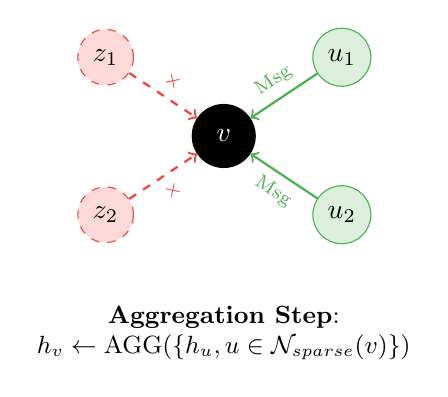
\begin{tikzpicture}
        % Center Node
        \node[circle, draw=black, fill=black, text=white, inner sep=2pt, minimum size=0.8cm] (v) at (0,0) {$v$};

        % Neighbors (Retained)
        \node[circle, draw=distillblue, fill=distillblue!20] (u1) at (1.5, 1) {$u_1$};
        \node[circle, draw=distillblue, fill=distillblue!20] (u2) at (1.5, -1) {$u_2$};

        % Neighbors (Pruned)
        \node[circle, draw=distillred, fill=distillred!20, dashed] (z1) at (-1.5, 1) {$z_1$};
        \node[circle, draw=distillred, fill=distillred!20, dashed] (z2) at (-1.5, -1) {$z_2$};

        % Messages (Arrows)
        \draw[->, thick, distillblue] (u1) -- node[midway, above, sloped, font=\scriptsize] {Msg} (v);
        \draw[->, thick, distillblue] (u2) -- node[midway, below, sloped, font=\scriptsize] {Msg} (v);

        % Pruned Messages
        \draw[->, thick, distillred, dashed] (z1) -- node[midway, above, sloped, font=\scriptsize] {$\times$} (v);
        \draw[->, thick, distillred, dashed] (z2) -- node[midway, below, sloped, font=\scriptsize] {$\times$} (v);

        % Context Label
        \node[align=center, font=\small] at (0, -2.5) {\textbf{Aggregation Step}:\\$h_v \leftarrow \text{AGG}(\{h_u, u \in \mathcal{N}_{sparse}(v)\})$};
    \end{tikzpicture}
    \caption{\textbf{Neighborhood Aggregation.} The GNN updates node $v$ by aggregating features from retained neighbors (green). Red dashed nodes represent neighbors removed by sparsification, reducing the computational cost of the aggregation step.}
    \label{fig:message_passing}
\end{figure}

\subsection{Sparsification Pipeline}

Our experimental pipeline, illustrated in Fig.~\ref{fig:pipeline}, consists of four stages: three for execution and one for evaluation.

\begin{enumerate}
    \item \textbf{Weight Computation.} For each edge $(u, v) \in E$, we compute a weight $w(u, v)$ that quantifies how ``important'' or ``redundant'' the edge is, according to the chosen scheme (Jaccard distance, Adamic-Adar-inspired weighting, or effective resistance).
    \item \textbf{Edge Filtering.} We remove edges based on the computed weights. For metric backbones, we retain edges that belong to the global metric backbone---those for which no shorter path of any length exists. Formally, we keep edge $(u,v)$ if and only if $w(u,v) = d_G(u,v)$, where $d_G$ denotes the shortest-path distance computed via all-pairs shortest paths (APSP). For spectral sparsification and random sampling, we sample edges with probabilities proportional to their effective resistances (or uniformly), targeting retention ratios $s \in \{0.3, 0.5, 0.7, 0.9\}$, where $s = |E'| / |E|$. For metric backbones, the sparsity is determined \emph{intrinsically} by the graph structure and the chosen weight function---it is an outcome, not an input parameter. To ensure fair comparison, we evaluate the spectral and random baselines at the specific sparsity level induced by the backbone for each dataset.
    \item \textbf{GNN Training.} We train the GNN on the sparsified graph $G' = (V, E')$ and evaluate classification performance. Crucially, the node features and labels remain unchanged; only the graph topology is modified.
    \item \textbf{Evaluation.} We quantify sparsification quality through the trade-off between compression and performance preservation. An ideal method maximizes sparsity (low $s$) while minimizing accuracy degradation. We define the \emph{accuracy retention} as the ratio of test accuracy on the sparsified graph to that on the original graph, $\text{Acc}(G') / \text{Acc}(G)$. The ``best'' method is the one that, at any given retention ratio $s$, achieves the highest accuracy retention---or equivalently, the one that achieves a target accuracy with the fewest edges.
\end{enumerate}

\paragraph{Ablation design.} To disentangle the effect of \emph{topology reduction} (removing edges) from the effect of \emph{edge reweighting} (assigning non-uniform importance to surviving edges), we adopt a factorial ablation design with four scenarios per configuration:
\begin{itemize}
    \item[\textbf{A.}] \emph{Full graph, binary weights}---the unmodified baseline.
    \item[\textbf{B.}] \emph{Sparse graph, binary weights}---isolates the pure effect of edge removal.
    \item[\textbf{C.}] \emph{Full graph, learned weights}---isolates the effect of edge reweighting without sparsification.
    \item[\textbf{D.}] \emph{Sparse graph, learned weights}---the full sparsification pipeline.
\end{itemize}
Comparing $\text{B} - \text{A}$ yields the \emph{structure effect} (accuracy change due to topology reduction alone), $\text{C} - \text{A}$ yields the \emph{weighting effect}, and $\text{D} - \text{A}$ yields the \emph{combined effect}. Note that for GraphSAGE, which does not support edge weights (see Section~\ref{sec:gnn_architectures}), scenarios C and D collapse to A and B respectively, and the weighting effect is zero by definition; only the structure effect is measurable. Each configuration is repeated across three random seeds to account for variance in initialization and optimization. We report the mean performance $\pm$ standard deviation to ensure reproducibility and robustness of the observed trends.

\begin{figure*}[t!]
    \centering
    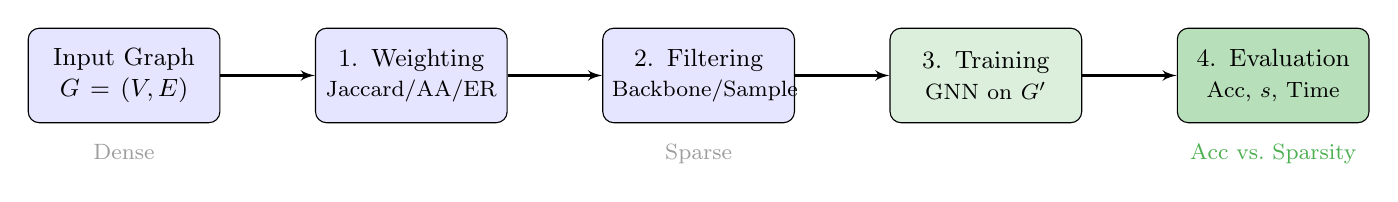
\begin{tikzpicture}[node distance=1.2cm, auto,
        block/.style={rectangle, draw, fill=blue!10, text width=2.2cm, text centered, rounded corners, minimum height=1.2cm, font=\small},
        line/.style={draw, -latex', thick}]

        % Nodes
        \node [block] (input) {Input Graph\\$G=(V, E)$};
        \node [block, right=of input] (weights) {1. Weighting\\{\footnotesize Jaccard/AA/ER}};
        \node [block, right=of weights] (filter) {2. Filtering\\{\footnotesize Backbone/Sample}};
        \node [block, right=of filter, fill=distillblue!20] (gnn) {3. Training\\{\footnotesize GNN on $G'$}};
        \node [block, right=of gnn, fill=distillblue!40] (eval) {4. Evaluation\\{\footnotesize Acc, $s$, Time}};

        % Arrows
        \path [line] (input) -- (weights);
        \path [line] (weights) -- (filter);
        \path [line] (filter) -- (gnn);
        \path [line] (gnn) -- (eval);

        % Labels
        \node [below=0.15cm of input, text=distillgrey, font=\footnotesize] {Dense};
        \node [below=0.15cm of filter, text=distillgrey, font=\footnotesize] {Sparse};
        \node [below=0.15cm of eval, text=distillblue, font=\footnotesize] {Acc vs.\ Sparsity};
    \end{tikzpicture}
    \caption{\textbf{The Sparsification Pipeline.} We compute importance scores for all edges, filter out those that violate the backbone constraint (or have low resistance), train the GNN on the resulting sparse structure, and evaluate the accuracy--sparsity trade-off.}
    \label{fig:pipeline}
\end{figure*}

\subsection{Jaccard-Based Weighting}

For citation networks, where nodes represent documents and edges represent citations, the structural similarity between the neighborhoods of connected nodes provides a meaningful notion of proximity. The intuition is straightforward: two papers that cite many of the same references are ``close'' in the intellectual landscape, regardless of whether they cite each other directly.

The \emph{Jaccard similarity} measures this neighborhood overlap as the ratio of shared neighbors to total neighbors:
\begin{equation}
    J(u, v) = \frac{|\mathcal{N}(u) \cap \mathcal{N}(v)|}{|\mathcal{N}(u) \cup \mathcal{N}(v)|}.
    \label{eq:jaccard_sim}
\end{equation}
A value of $J(u,v) = 1$ means $u$ and $v$ have identical neighborhoods; $J(u,v) = 0$ means they share no neighbors at all. To apply the metric backbone framework, we need to convert this similarity into an edge \emph{weight} (dissimilarity). A natural choice would be the Jaccard distance $d_J = 1 - J$, but this is a proper metric satisfying the triangle inequality everywhere---meaning the direct edge is \emph{always} a shortest path, no edge would ever be classified as semi-metric, and the backbone would retain the entire graph. To obtain meaningful sparsification, we apply the \emph{proximity-to-distance} transformation introduced by Simas et al.~\cite{simas2021}. First, we normalize the Jaccard similarities to a \emph{proximity} $p(u,v) \in (0, 1]$ by dividing by the maximum observed value. Then we convert to an edge cost via the isomorphic transformation:
\begin{equation}
    w_J(u, v) = \frac{1}{p_J(u, v)} - 1, \quad \text{where } p_J(u,v) = \frac{J(u,v)}{\max_{(i,j) \in E} J(i,j)}.
    \label{eq:jaccard_weight}
\end{equation}

This mapping sends high-similarity edges to short distances ($p \approx 1 \Rightarrow w \approx 0$) and low-similarity edges to large distances ($p \to 0 \Rightarrow w \to \infty$), while satisfying two critical properties: it is monotone decreasing, and---unlike the Jaccard distance $1 - J$---it deliberately violates the triangle inequality, which is what enables the backbone to detect redundant edges. Consider an edge $(u,v)$ with low overlap ($J(u,v) \approx 0$, hence $w_J(u,v) \gg 1$). If there exists an intermediate node $z$ sharing many neighbors with both $u$ and $v$---so that $J(u,z)$ and $J(z,v)$ are both large, making $w_J(u,z)$ and $w_J(z,v)$ both small---then the indirect path $u \to z \to v$ has total weight $w_J(u,z) + w_J(z,v) < w_J(u,v)$. The direct edge is costlier than the detour, the geodesic distance satisfies $d_G(u,v) < w_J(u,v)$, and the backbone removes it.

The backbone thus retains edge $(u,v)$ only when its direct semantic link is stronger (lower weight) than any indirect composite path through the rest of the network. Edges that survive this test represent irreplaceable structural connections; those that are removed can be ``explained away'' by stronger indirect paths through shared neighbors.

\paragraph{Why Jaccard is well-suited for citation networks.} The underlying Jaccard similarity is a \emph{normalized} measure of \emph{relative} neighborhood overlap, bounded in $[0, 1]$ regardless of absolute node degrees. This normalization is particularly advantageous for citation networks such as Cora and PubMed, where degree distributions are relatively \emph{homogeneous}: academic papers typically cite a limited number of references (constrained by publication norms), resulting in moderate and comparable node degrees across the graph. In such settings, a high Jaccard similarity indicates genuine \emph{semantic proximity}---papers sharing many citations likely address related topics within the same research subfield. Because the similarity reflects the \emph{proportion} of shared context rather than raw counts, the resulting inverse weights produce meaningful comparisons even when nodes have slightly different degrees. For GNN-based node classification, where the goal is to predict research categories, this semantic proximity translates directly into label coherence: nodes with high Jaccard similarity are likely to share the same class label, and the corresponding low-weight edges are preferentially retained by the backbone---making the Jaccard-based backbone a principled choice for preserving classification-relevant structure.

\subsection{Adamic-Adar-Inspired Weighting}\label{sec:adamic_adar}

Social networks exhibit fundamentally different topological properties than citation networks. They are characterized by \emph{scale-free} degree distributions, in which the probability $P(k)$ of observing a node with degree $k$ follows a power law:
\begin{equation}
    P(k) \propto k^{-\gamma},
    \label{eq:power_law}
\end{equation}
where $\gamma$ is the power-law exponent. The heavy tail of this distribution implies that, while the vast majority of nodes have modest connectivity, a small number of \emph{hub} nodes accumulate a disproportionately large number of connections. Networks such as Flickr, Twitter, and Facebook are dominated by these high-degree hubs---celebrities, influencers, and viral content creators---who connect to millions of users.

In this setting, the Jaccard distance has a critical blind spot: it treats all common neighbors equally, regardless of their degree. Sharing a hub neighbor is \emph{not informative}---a celebrity followed by millions of users provides no signal about the relationship between two specific followers. Conversely, sharing a \emph{low-degree} neighbor is a strong signal of genuine community membership: if two users both follow a niche expert with only a handful of connections, they likely share specific interests or belong to the same specialized community.

The \emph{Adamic-Adar index}~\cite{adamic2003} captures precisely this intuition by mathematically penalizing high-degree common neighbors via an inverse logarithmic weighting:
\begin{equation}
    \text{AA}(u, v) = \sum_{z \in \mathcal{N}(u) \cap \mathcal{N}(v)} \frac{1}{\log |\mathcal{N}(z)|}.
    \label{eq:adamic_adar}
\end{equation}

Each common neighbor $z$ contributes inversely to the logarithm of its degree. A common neighbor with degree 3 contributes $1/\log 3 \approx 0.91$, while a hub with degree 10{,}000 contributes only $1/\log 10000 \approx 0.11$---an eight-fold reduction. The index thus emphasizes connections through selective, low-degree nodes while suppressing the noise introduced by ubiquitous hubs.

\paragraph{Empirical superiority in social link prediction.} The theoretical motivation for Adamic-Adar is supported by extensive empirical evidence. In their seminal study of link prediction across diverse social networks, Liben-Nowell and Kleinberg~\cite{liben2007} demonstrated that the Adamic-Adar index consistently outperforms simpler similarity measures---including the Jaccard coefficient and common neighbors---on networks with heterogeneous degree distributions. The inverse log-degree weighting allows Adamic-Adar to distinguish between ``weak'' connections through hubs and ``strong'' connections through low-degree intermediaries. For GNN-based node classification on social networks, where class labels often correspond to interest groups or communities, this distinction is precisely what matters: the Adamic-Adar weighting prioritizes edges that reflect meaningful community structure over edges that merely reflect hub connectivity.

\paragraph{Why the Adamic-Adar distance cannot be used directly.} A natural approach would be to convert the Adamic-Adar similarity into a distance---for instance via $d(u,v) = 1/(1 + \text{AA}(u,v))$---and apply the metric backbone framework directly. However, the Adamic-Adar index, when properly transformed into a distance, forms a valid metric. This is precisely the problem: when we compute all-pairs shortest paths, every direct edge weight $d(u,v)$ equals the geodesic distance $d_G(u,v)$, so no edge is ever classified as semi-metric. The backbone retains the \emph{entire graph}, and the sparsification is trivial---rendering the method useless for our purposes.

\paragraph{Proximity-to-distance transformation.} To overcome this limitation, we apply the same proximity-to-distance transformation from Simas et al.~\cite{simas2021} as for the Jaccard coefficient. First, we normalize the Adamic-Adar scores to a proximity $p_{\text{AA}}(u,v) \in (0, 1]$, then convert to costs:
\begin{equation}
    w_{\text{AA}}(u, v) = \frac{1}{p_{\text{AA}}(u, v)} - 1, \quad p_{\text{AA}}(u,v) = \frac{\text{AA}(u,v)}{\max_{(i,j)} \text{AA}(i,j)}.
    \label{eq:aa_weight}
\end{equation}
We then apply the APSP-based backbone extraction: we compute shortest-path distances $d_G(u,v)$ using Dijkstra's algorithm and remove edge $(u,v)$ when:
\begin{equation}
    w_{\text{AA}}(u, v) > d_G(u, v).
    \label{eq:aa_violation}
\end{equation}
This mirrors the Jaccard case: edges between nodes with high Adamic-Adar similarity receive low weights, while edges between weakly connected nodes receive very high weights. The transformation is not a proper metric, enabling the backbone to detect semi-metric edges. Edges with zero Adamic-Adar score (no common neighbors) are assigned a small positive floor before normalization.

\begin{figure}[t!]
    \centering
    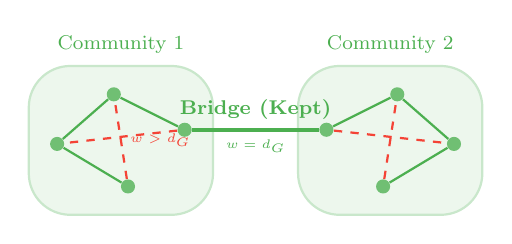
\begin{tikzpicture}[scale=0.9, transform shape]
        % Community 1 (Left) - Dense
        \node[circle, fill=distillblue!80, inner sep=2pt] (a1) at (0, 0.5) {};
        \node[circle, fill=distillblue!80, inner sep=2pt] (a2) at (-0.8, -0.2) {};
        \node[circle, fill=distillblue!80, inner sep=2pt] (a3) at (0.2, -0.8) {};
        \node[circle, fill=distillblue!80, inner sep=2pt] (a4) at (1, 0) {};

        % Community 2 (Right) - Dense
        \node[circle, fill=distillblue!80, inner sep=2pt] (b1) at (4, 0.5) {};
        \node[circle, fill=distillblue!80, inner sep=2pt] (b2) at (4.8, -0.2) {};
        \node[circle, fill=distillblue!80, inner sep=2pt] (b3) at (3.8, -0.8) {};
        \node[circle, fill=distillblue!80, inner sep=2pt] (b4) at (3, 0) {};

        % Background blobs for communities
        \begin{pgfonlayer}{background}
            \draw[fill=distillblue!10, draw=distillblue!30, thick, rounded corners=15pt] (-1.2, -1.2) rectangle (1.4, 0.9);
            \draw[fill=distillblue!10, draw=distillblue!30, thick, rounded corners=15pt] (2.6, -1.2) rectangle (5.2, 0.9);
        \end{pgfonlayer}

        % Labels
        \node[text=distillblue, font=\footnotesize] at (0.1, 1.2) {Community 1};
        \node[text=distillblue, font=\footnotesize] at (3.9, 1.2) {Community 2};

        % Edges Community 1
        \draw[thick, distillblue] (a1) -- (a2);
        \draw[thick, distillblue] (a2) -- (a3);
        \draw[thick, distillblue] (a1) -- (a4);
        \draw[thick, distillred, dashed] (a3) -- node[midway, right, font=\tiny] {$w > d_G$} (a1); % Pruned
        \draw[thick, distillred, dashed] (a4) -- (a2); % Pruned

        % Edges Community 2
        \draw[thick, distillblue] (b1) -- (b2);
        \draw[thick, distillblue] (b2) -- (b3);
        \draw[thick, distillblue] (b4) -- (b1);
        \draw[thick, distillred, dashed] (b3) -- (b1); % Pruned
        \draw[thick, distillred, dashed] (b4) -- (b2); % Pruned

        % Inter-community Bridge (Kept)
        \draw[ultra thick, distillblue] (a4) -- node[midway, above, font=\footnotesize\bfseries] {Bridge (Kept)} node[midway, below, font=\tiny] {$w = d_G$} (b4);

    \end{tikzpicture}
    \caption{\textbf{Metric Backbone in Community Graphs.} The APSP-based metric backbone efficiently prunes redundant intra-community edges (red dashed lines) while preserving critical inter-community bridges (solid blue lines), reducing density while maintaining global community structure~\cite{dreveton2024}.}
    \label{fig:backbone_communities}
\end{figure}

The semi-metric edges under this scheme---those where $w(u,v) > d_G(u,v)$---concentrate around high-degree hub nodes, and this is precisely the desired behavior. An edge $(u,v)$ whose only common neighbors are hubs receives a low Adamic-Adar score, hence a low proximity $p_{\text{AA}}(u,v)$ and a high cost $w_{\text{AA}}(u,v) \gg 1$. If a detour $u \to z \to v$ exists through a low-degree community member $z$---who contributes strongly to both $\text{AA}(u,z)$ and $\text{AA}(z,v)$, yielding high proximity and low costs on both legs---then the indirect path is cheaper and the direct hub-dependent edge is pruned. In other words, the backbone removes weak edges whose connectivity relies on ubiquitous hubs, in favor of stronger, lower-cost paths through local community members. The result is a sparser graph that better reflects the mesoscale community structure of networks with heavy-tailed degree distributions.

\subsection{Effective Resistance}

The \emph{effective resistance} offers a complementary, spectral perspective on edge importance. The intuition is borrowed from electrical network theory: imagine replacing every edge in the graph with a unit resistor, then measuring the resistance between two nodes $u$ and $v$ by injecting a unit current at $u$ and extracting it at $v$. The effective resistance $R_{\text{eff}}(u,v)$ is the resulting voltage difference.

Formally, it is defined in terms of the pseudoinverse $L^+$ of the graph Laplacian $L$:
\begin{equation}
    R_{\text{eff}}(u, v) = L^+_{uu} + L^+_{vv} - 2L^+_{uv},
    \label{eq:effective_resistance}
\end{equation}
where $L^+_{ij}$ denotes the $(i,j)$-entry of $L^+$.

What does this quantity capture? An edge with \emph{high} effective resistance is a ``bridge'': removing it would significantly alter the flow of information (or current) through the network, because few alternative paths exist. An edge with \emph{low} effective resistance is deeply embedded in a dense region with many parallel paths---its removal barely changes the network's connectivity. Spectral sparsification exploits this by sampling edges with probabilities proportional to their effective resistances, ensuring that bridge-like edges are retained while redundant edges in dense regions are pruned.

\paragraph{ER weighting for backbone extraction.} The effective resistance is a proper metric on graphs---it satisfies the triangle inequality by construction. As with the Jaccard distance, this means that using $R_{\text{eff}}$ directly as edge weights would make every edge metric, and the backbone would retain the entire graph. We therefore apply the proximity-to-distance transformation~\cite{simas2021}: since $R_{\text{eff}}$ is inherently a \emph{distance} (higher values indicate more distant nodes), we first invert it to obtain a similarity $s_{\text{ER}}(u,v) = 1 / R_{\text{eff}}(u,v)$, normalize to proximity, and then convert to costs:
\begin{equation}
    w_{\text{ER}}(u, v) = \frac{1}{p_{\text{ER}}(u, v)} - 1, \quad p_{\text{ER}}(u,v) = \frac{s_{\text{ER}}(u,v)}{\max_{(i,j)} s_{\text{ER}}(i,j)}.
    \label{eq:er_weight}
\end{equation}
Edges with low effective resistance (deeply embedded in dense regions) have high similarity $s_{\text{ER}}$, hence high proximity and low weight, while bridges with high resistance have low similarity, low proximity, and thus high weight. The transformation breaks the triangle inequality, enabling the backbone to identify semi-metric edges. In practice, however, the ER-based backbone retains a very large fraction of edges on sparse citation networks (${\sim}99\%$), because bridge edges---despite their high weight---have no alternative paths, and dense-region edges have very low weights that no detour can undercut.

\paragraph{Connection to Graph Signal Processing.} The spectral sparsification framework has an elegant interpretation in terms of graph signal processing. The quadratic form $\mathbf{x}^\top L \mathbf{x}$, which spectral sparsifiers preserve (cf.\ Eq.~\eqref{eq:spectral_sparsifier}), measures the \emph{smoothness} of a signal $\mathbf{x}$ defined on the graph vertices:
\begin{equation}
    \mathbf{x}^\top L \mathbf{x} = \sum_{(u,v) \in E} (x_u - x_v)^2.
    \label{eq:signal_smoothness}
\end{equation}
This quantity computes the total squared variation of the signal across edges---a signal is ``smooth'' if connected nodes carry similar values. For GNNs, this is precisely what matters: the message-passing mechanism can be viewed as iteratively smoothing node features over the graph, where the ``energy'' of the signal (measured by this quadratic form) governs how information diffuses. By ensuring that $(1 - \varepsilon) \, \mathbf{x}^\top L_G \mathbf{x} \leq \mathbf{x}^\top L_H \mathbf{x} \leq (1 + \varepsilon) \, \mathbf{x}^\top L_G \mathbf{x}$ for all signals $\mathbf{x}$, spectral sparsifiers guarantee that feature diffusion on the sparse graph $H$ faithfully approximates diffusion on the original graph $G$. In other words, the GNN can still effectively propagate and aggregate features across the sparsified structure, because the fundamental ``energy landscape'' that governs signal flow has been preserved.

\paragraph{Computational Complexity.} Computing exact effective resistances requires the pseudoinverse of the $n \times n$ Laplacian, at a cost of $\mathcal{O}(n^3)$. This is prohibitive for large graphs. The approximate method based on the Johnson-Lindenstrauss transform (JLT) reduces this to $\mathcal{O}(m \log n)$ by projecting the Laplacian pseudoinverse onto a low-dimensional random subspace~\cite{spielman2011}. In our implementation, we employ the approximate method to ensure scalability to the larger datasets in our study.

\subsection{Summary of Methods}

Table~\ref{tab:methods_summary} summarizes the sparsification methods considered in this study, along with their computational complexity and the type of structural property they preserve.

\begin{table}[t!]
\caption{Summary of Sparsification Methods}
\begin{center}
\begin{tabular}{lccc}
\toprule
\textbf{Method} & \textbf{Complexity} & \textbf{Preserves} \\
\midrule
Random & $\mathcal{O}(m)$ & None (baseline) \\
Jaccard Backbone & $\mathcal{O}(m \cdot \bar{d})$ & Metric structure \\
Adamic-Adar Backbone & $\mathcal{O}(m \cdot \bar{d})$ & Metric structure \\
ER Backbone & $\mathcal{O}(m \log n)$ & Metric structure \\
\bottomrule
\end{tabular}
\label{tab:methods_summary}
\end{center}
\end{table}

Here $\bar{d}$ denotes the average degree, reflecting the cost of computing neighborhood intersections for each edge.

%% ========================================================================
\section{Experimental Setup}\label{sec:experimental_setup}
%% ========================================================================

\subsection{Datasets}

We evaluate the sparsification methods on twelve benchmark datasets from PyTorch Geometric, deliberately chosen to span a broad range of domains, scales, and structural properties. Table~\ref{tab:datasets} summarizes their statistics. A key design choice is the inclusion of both \emph{homophilic} networks (where connected nodes tend to share the same label) and \emph{heterophilic} networks (where connected nodes often have different labels), allowing us to assess whether sparsification methods interact differently with these contrasting regimes.

\begin{table}[t!]
\caption{Dataset Statistics}
\begin{center}
\small
\begin{tabular}{lrrrcrc}
\toprule
\textbf{Dataset} & $|V|$ & $|E|$ & \textbf{Feat.} & $C$ & $h$ & $\bar{d}$ \\
\midrule
\multicolumn{7}{l}{\textit{Citation networks}} \\
Cora & 2{,}708 & 5{,}278 & 1{,}433 & 7 & 0.81 & 3.90 \\
CiteSeer & 3{,}327 & 4{,}552 & 3{,}703 & 6 & 0.74 & 2.74 \\
PubMed & 19{,}717 & 44{,}324 & 500 & 3 & 0.80 & 4.50 \\
DBLP & 17{,}716 & 52{,}867 & 1{,}639 & 4 & 0.83 & 5.97 \\
Cora\_ML & 2{,}995 & 8{,}158 & 2{,}879 & 7 & 0.79 & 5.45 \\
\midrule
\multicolumn{7}{l}{\textit{WebKB networks (heterophilic)}} \\
Cornell & 183 & 149 & 1{,}703 & 5 & 0.13 & 1.63 \\
Texas & 183 & 162 & 1{,}703 & 5 & 0.11 & 1.77 \\
Wisconsin & 251 & 257 & 1{,}703 & 5 & 0.20 & 2.05 \\
\midrule
\multicolumn{7}{l}{\textit{Wikipedia networks (heterophilic)}} \\
Chameleon & 2{,}277 & 18{,}050 & 2{,}325 & 5 & 0.24 & 15.85 \\
Squirrel & 5{,}201 & 108{,}536 & 2{,}089 & 5 & 0.22 & 41.74 \\
\midrule
\multicolumn{7}{l}{\textit{Other domains}} \\
Actor & 7{,}600 & 15{,}009 & 932 & 5 & 0.22 & 3.95 \\
PPI & 1{,}767 & 16{,}159 & 50 & 121$^\dagger$ & 0.36 & 18.29 \\
\bottomrule
\multicolumn{7}{l}{\footnotesize $C$: classes. $h$: edge homophily. $\bar{d}$: avg.\ degree. $^\dagger$Multi-label.}
\end{tabular}
\label{tab:datasets}
\end{center}
\end{table}

\paragraph{Citation networks.} Cora, CiteSeer, PubMed, DBLP, and Cora\_ML are citation graphs where nodes represent publications and edges represent citation links. Node features are bag-of-words vectors derived from paper abstracts, and labels correspond to research subfields. These networks exhibit high homophily ($h > 0.7$), relatively homogeneous degree distributions, and sparse binary features---properties that make them well-suited to the Jaccard distance backbone. They range from small (Cora, 2{,}708 nodes) to medium-scale (PubMed, DBLP, ${\sim}$20K nodes), allowing us to assess sparsification across different graph sizes within the same domain.

\paragraph{Heterophilic benchmarks.} The WebKB networks (Cornell, Texas, Wisconsin) and Wikipedia networks (Chameleon, Squirrel) exhibit low homophily ($h < 0.25$), meaning that connected nodes frequently belong to \emph{different} classes. These datasets pose a distinct challenge for sparsification: methods that aggressively prune edges based on neighborhood similarity may inadvertently remove the cross-class edges that heterophilic GNNs rely upon. The WebKB graphs are notably small (${\sim}$200 nodes), while Squirrel is relatively dense (${\sim}$108K edges for 5{,}201 nodes), providing contrasting sparsification regimes.

\paragraph{Actor and PPI.} The Actor co-occurrence network and the Protein-Protein Interaction (PPI) graph extend our evaluation beyond citation and web domains. Actor is a heterophilic social network ($h = 0.22$) where nodes represent actors and edges co-occurrence in Wikipedia pages. PPI is a biological network with dense, low-dimensional features and multi-label classification, testing whether sparsification methods generalize to non-textual feature spaces.

\subsection{GNN Architectures}\label{sec:gnn_architectures}

We employ three representative GNN architectures that instantiate the message-passing framework in different ways, each offering a distinct aggregation strategy that interacts differently with sparsification.

\paragraph{Graph Convolutional Network (GCN).} Introduced by Kipf and Welling~\cite{kipf2017}, GCN implements the message-passing steps as follows. In the \emph{message computation} step, each neighbor's features are linearly transformed by a shared weight matrix $\mathbf{W}^{(k)}$. In the \emph{aggregation} step, messages are combined by normalized summation, where the normalization factor $\tilde{D}^{-1/2} \tilde{A} \, \tilde{D}^{-1/2}$ ensures that nodes with many neighbors do not dominate. Finally, the \emph{update} step applies a nonlinear activation. The full layer operation is:
\begin{equation}
    \mathbf{H}^{(k+1)} = \sigma\!\left(\tilde{D}^{-1/2} \tilde{A} \, \tilde{D}^{-1/2} \mathbf{H}^{(k)} \mathbf{W}^{(k)}\right),
    \label{eq:gcn}
\end{equation}
where $\tilde{A} = A + I_n$ is the adjacency matrix augmented with self-loops (so that each node also retains its own features), $\tilde{D}$ is the corresponding degree matrix, and $\sigma$ is a nonlinear activation such as ReLU.

The key property of GCN for our purposes is that the aggregation weights are \emph{fixed} by the graph structure. Every neighbor contributes equally (up to degree normalization), which means that GCN cannot compensate for removed edges by up-weighting surviving neighbors. This makes GCN performance particularly sensitive to the choice of sparsification method.

\paragraph{GraphSAGE.} Introduced by Hamilton et al.~\cite{hamilton2017}, GraphSAGE (\emph{SAmple and aggreGatE}) was designed for \emph{inductive} learning on large-scale graphs. Unlike GCN, which requires the full graph Laplacian at training time, GraphSAGE generates node embeddings by sampling and aggregating features from a fixed-size neighborhood. In its mean-aggregator variant (which we adopt), the layer operation is:
\begin{equation}
    \mathbf{h}_v^{(k)} = \sigma\!\bigg(\mathbf{W}^{(k)} \cdot \textsc{Mean}\!\Big(\big\{\mathbf{h}_u^{(k-1)} : u \in \mathcal{N}(v) \cup \{v\}\big\}\Big)\bigg).
    \label{eq:sage}
\end{equation}
A distinctive property of GraphSAGE is that it does \emph{not} natively support edge weights: the mean aggregator treats all neighbors equally, and any edge importance information computed during sparsification is discarded at training time. This means that for GraphSAGE, only the \emph{topology} of the sparsified graph matters---the weighting effect (scenario C in our ablation) is absent, isolating the pure structural effect of edge removal.

\paragraph{Graph Attention Network (GAT).} Introduced by Veli\v{c}kovi\'{c} et al.~\cite{velickovic2018}, GAT replaces GCN's fixed aggregation weights with \emph{learned attention coefficients}, allowing the model to dynamically decide how much to ``listen'' to each neighbor. The process unfolds in three stages:

\begin{enumerate}
    \item \emph{Message computation:} Each node's features are linearly transformed by a shared weight matrix $\mathbf{W}$.
    \item \emph{Attention scoring:} For each edge $(u, v)$, a scalar attention score is computed by concatenating the transformed features of $u$ and $v$ and passing them through a learnable attention mechanism:
    \begin{equation}
        e_{uv} = \text{LeakyReLU}\!\Big(\mathbf{a}^\top \big[\mathbf{W}\mathbf{h}_u \,\big\|\, \mathbf{W}\mathbf{h}_v\big]\Big),
        \label{eq:gat_score}
    \end{equation}
    where $\|$ denotes concatenation and $\mathbf{a}$ is a learnable attention vector.
    \item \emph{Aggregation with normalized attention:} The raw scores are normalized across all neighbors of $v$ via softmax, producing attention weights $\alpha_{uv}$ that sum to one:
    \begin{equation}
        \alpha_{uv} = \frac{\exp(e_{uv})}{\sum_{z \in \mathcal{N}(v)} \exp(e_{vz})}.
        \label{eq:gat_attention}
    \end{equation}
\end{enumerate}

Because GAT can learn to assign different importances to different neighbors, it may be more robust to sparsification than GCN: if a removed edge was already receiving low attention weight, its absence has minimal impact. Conversely, if sparsification removes edges that the attention mechanism deemed important, the performance degradation could be more severe.

\subsection{Evaluation Metrics}

We evaluate each sparsification method along four complementary dimensions:
\begin{itemize}
    \item \textbf{Classification Accuracy.} Test set accuracy on the node classification task, averaged over three random seeds ($\{42, 123, 456\}$) and reported with 95\% confidence intervals. We report both absolute accuracy and the \emph{accuracy drop} $\Delta = \text{Acc}(G) - \text{Acc}(G')$ relative to the unsparsified baseline.
    \item \textbf{Sparsity Ratio.} The fraction of edges retained, $s = |E'| / |E|$, evaluated at four levels: $s \in \{0.3, 0.5, 0.7, 0.9\}$. For metric backbones, the retention ratio is determined by the graph's intrinsic structure rather than a user-specified threshold.
    \item \textbf{Computational Cost.} Wall-clock time decomposed into \emph{preprocessing time} (weight computation and edge filtering) and \emph{training time} (GNN optimization on the sparsified graph). The total cost of sparsification is justified only when preprocessing overhead is amortized by reduced per-epoch training time.
    \item \textbf{Structural Preservation.} We additionally measure the degree to which sparsified graphs preserve topological properties relevant to GNNs, including clustering coefficient ratio, algebraic connectivity preservation ($\lambda_2(G') / \lambda_2(G)$), and geodesic distance preservation (fraction of sampled node pairs whose shortest-path distance is unchanged).
\end{itemize}

\subsection{Research Questions}

Our experimental evaluation is designed to address the following research questions:

\begin{enumerate}
    \item \textbf{Accuracy--sparsity trade-off.} Which sparsification strategies best preserve GNN classification accuracy as the sparsity ratio decreases? Is there a saturation effect beyond which further sparsification leads to rapid performance degradation?
    \item \textbf{Computational efficiency.} How does the choice of sparsification method influence the end-to-end training time, accounting for both the sparsification preprocessing cost and the reduced per-epoch training cost?
    \item \textbf{Dataset dependence.} Do different graph types (citation vs.\ social) respond differently to metric-based vs.\ spectral sparsification? In particular, does the Adamic-Adar-inspired backbone outperform the Jaccard backbone on social networks, and vice versa?
    \item \textbf{Structure preservation.} To what extent do the sparsified graphs preserve topological properties relevant to GNNs, such as degree distribution, clustering coefficient, and connected component structure?
\end{enumerate}

%% ========================================================================
%% Bibliography
%% ========================================================================

\begin{thebibliography}{00}

\bibitem{kipf2017} T.~N. Kipf and M.~Welling, ``Semi-supervised classification with graph convolutional networks,'' in \emph{Proc. Int. Conf. Learn. Represent. (ICLR)}, 2017.

\bibitem{spielman2008} D.~A. Spielman and N.~Srivastava, ``Graph sparsification by effective resistances,'' in \emph{Proc. 40th Annu. ACM Symp. Theory Comput. (STOC)}, 2008, pp.~563--568.

\bibitem{spielman2011} D.~A. Spielman and S.~H. Teng, ``Spectral sparsification of graphs,'' \emph{SIAM J. Comput.}, vol.~40, no.~4, pp.~981--1025, 2011.

\bibitem{dreveton2024} M.~Dreveton, C.~Chucri, M.~Grossglauser, and P.~Thiran, ``Why the metric backbone preserves community structure,'' in \emph{Proc. Adv. Neural Inf. Process. Syst. (NeurIPS)}, 2024.

\bibitem{hamilton2017} W.~L. Hamilton, R.~Ying, and J.~Leskovec, ``Inductive representation learning on large graphs,'' in \emph{Proc. Adv. Neural Inf. Process. Syst. (NeurIPS)}, 2017, pp.~1024--1034.

\bibitem{velickovic2018} P.~Veli\v{c}kovi\'{c} et al., ``Graph attention networks,'' in \emph{Proc. Int. Conf. Learn. Represent. (ICLR)}, 2018.

\bibitem{adamic2003} L.~A. Adamic and E.~Adar, ``Friends and neighbors on the web,'' \emph{Soc. Netw.}, vol.~25, no.~3, pp.~211--230, 2003.

\bibitem{chung1997} F.~R.~K. Chung, \emph{Spectral Graph Theory}, Amer. Math. Soc., 1997.

\bibitem{rong2020} Y.~Rong, W.~Huang, T.~Xu, and J.~Huang, ``DropEdge: Towards deep graph convolutional networks on node classification,'' in \emph{Proc. Int. Conf. Learn. Represent. (ICLR)}, 2020.

\bibitem{liben2007} D.~Liben-Nowell and J.~Kleinberg, ``The link-prediction problem for social networks,'' \emph{J. Am. Soc. Inf. Sci. Technol.}, vol.~58, no.~7, pp.~1019--1031, 2007.

\bibitem{zheng2020} C.~Zheng et al., ``Robust graph representation learning via neural sparsification,'' in \emph{Proc. Int. Conf. Mach. Learn. (ICML)}, 2020.

\bibitem{simas2021} T.~Simas, R.~Chattopadhyay, C.~Huepe, and L.~M. Rocha, ``An overview of the distance backbone of complex networks: properties, models, and algorithms,'' \emph{J. Complex Netw.}, vol.~9, no.~6, cnab021, 2021.

\end{thebibliography}

\end{document}
